\chapter{Results and discussion}

\section{RGCN is able to accurately predict expected water solubility}


The resulting ten RGCN models, each with a different seed, have comparable results 
(\cref{fig:training_history}). 
Performance of the training data is relatively good, yielding an average $R^2$ 
of $0.96$ and an average mean squared error (MSE) of $0.074$. The model has a 
similar $R^2$ for the validation data ($0.92$), however, larger errors are made 
(MSE is $0.340$). The same holds for the test data set, which has an $R^2$ of 
$0.91$ and an MSE of $0.32$. Considering that most experimental data have an RMSE 
between $0.6$ and $0.7$ log(mol/L),\cite{palmer2014experimental} 
it can be concluded that the resulting model can predict water solubility of small 
molecules with decent performance.

% \begin{figure}[h]
%     \centering
%     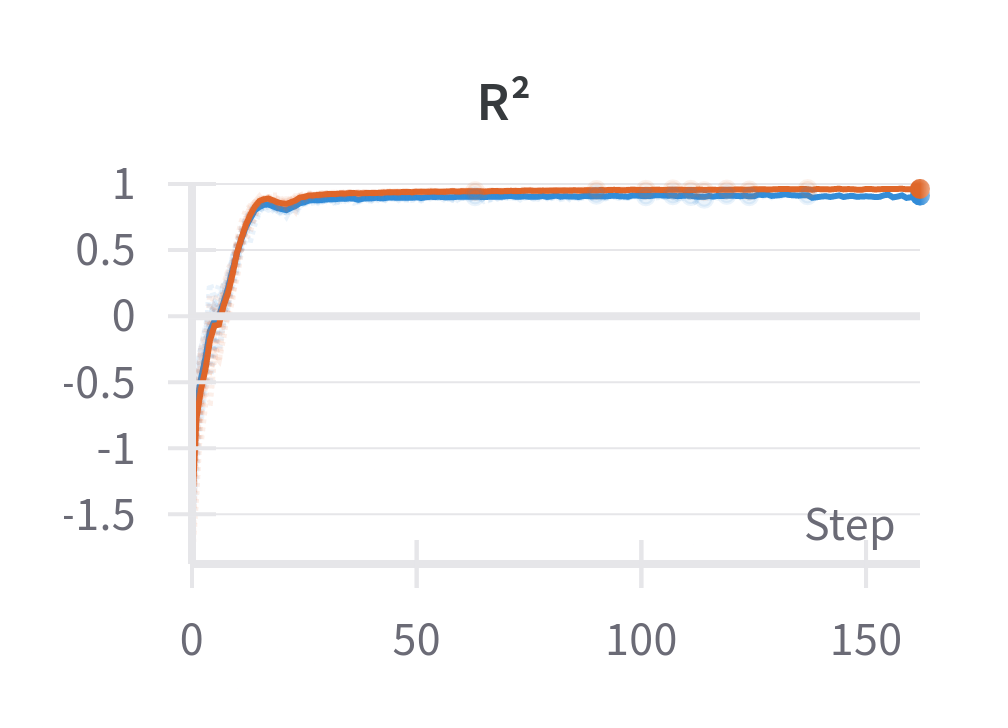
\includegraphics[scale=0.20]{rgcn_r2.png}
%     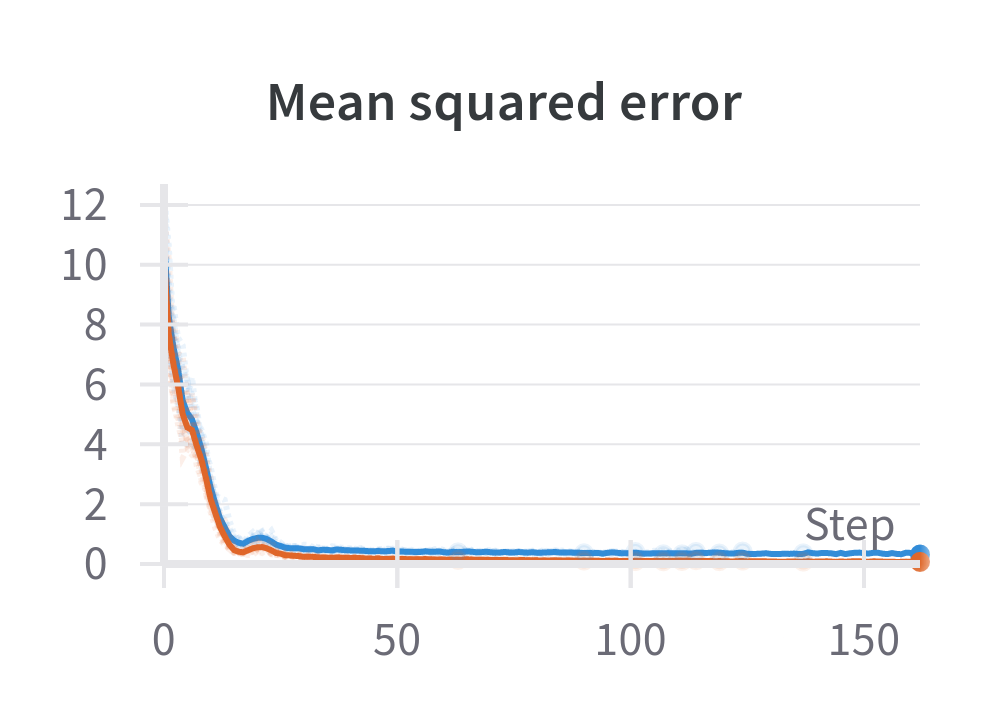
\includegraphics[scale=0.20]{rgcn_mse.png}
%     \caption{Average Mean squared error (left) and $R^2$ (right) of train (orange) and validation 
%     (blue) data during model training over the ten RGCN models, each trained using a different 
%     seed. Both metrics show a good model performance and no overfitting.}
% \end{figure}


\begin{figure}[h]
    \centering
    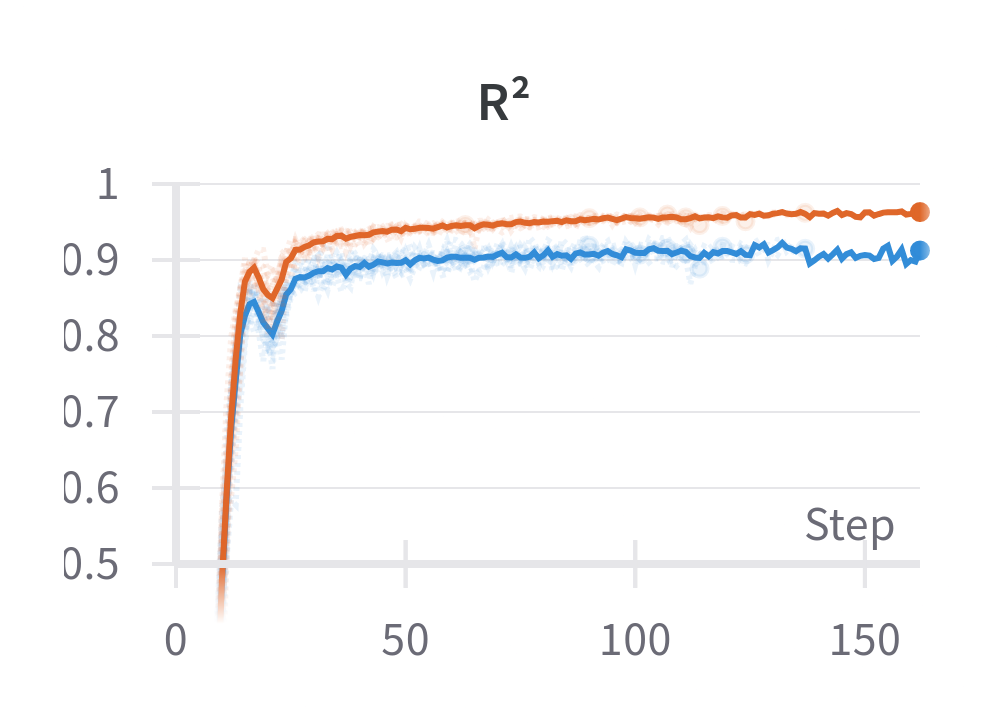
\includegraphics[scale=0.20]{rgcn_r2_zoomed.png}
    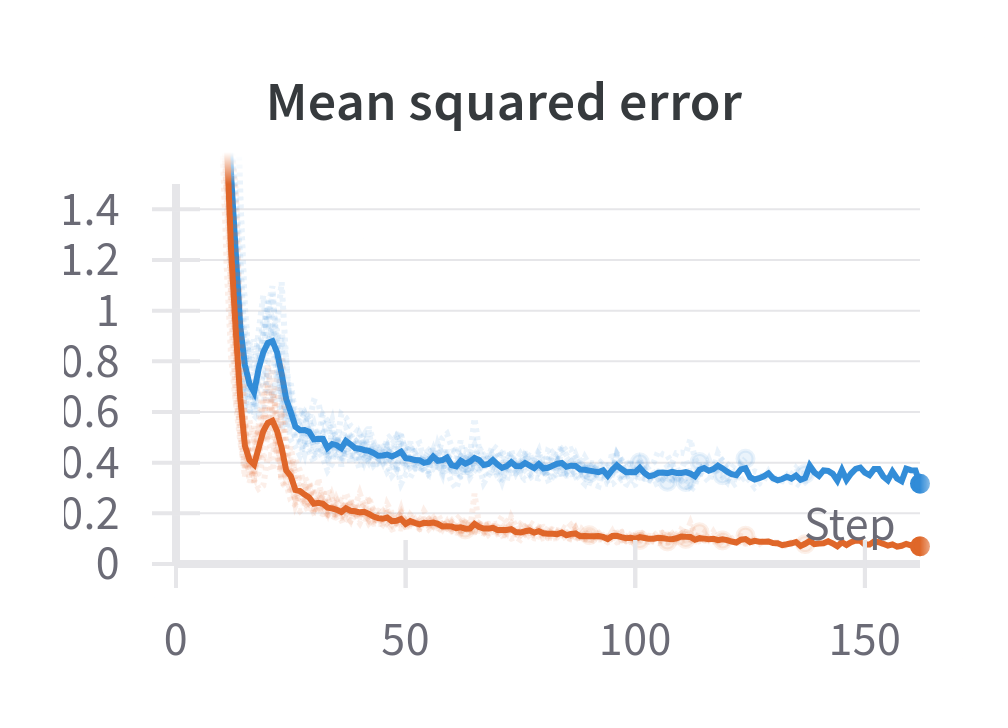
\includegraphics[scale=0.20]{rgcn_mse_zoomed.png}
    \caption{Average $R^2$ (left) and mean squared error (right) of train (orange) and validation 
    (blue) data during model training over the ten RGCN models, each trained using a different 
    seed. Both metrics show a good model performance and no overfitting. }
    \label{fig:training_history}
\end{figure}


Currently, it is questionable whether the ML model effectively learns chemistry and 
if wrong predictions may be explained by chemically incorrect reasoning of the model. 
To address this, different attribution methods (SME, Shapley value and HN value) are 
compared to each other and with chemical theory. It should be noted that these attribution 
methods can reveal insights into the chemical reasoning of the model, but are not necessarily 
causal. This means that if the attributions show inconsistency with chemical theory, other 
factors could also influence the wrong prediction.


\section{Different attribution methods can result in different explanations}


The attribution values sign usually shows an agreement with expectations from 
chemistry (\cref{fig:attribution_distribution_fg}). Groups that positively affect the polarity of a molecule have a 
positive attribution, while unfavorable functional groups for water solubility 
have a negative attribution. The median of HN values also shows a correct 
relationship between the functional groups. Hydroxyl groups are hydrogen bond 
acceptors and donors, so it has a superior influence on water solubility than 
a methyl ester that can only accept hydrogen bonds. Also, ethoxy has a lower 
HN value than methoxy, which is due to the larger carbon chain of ethoxy.


\begin{figure}[h]
    \centering
    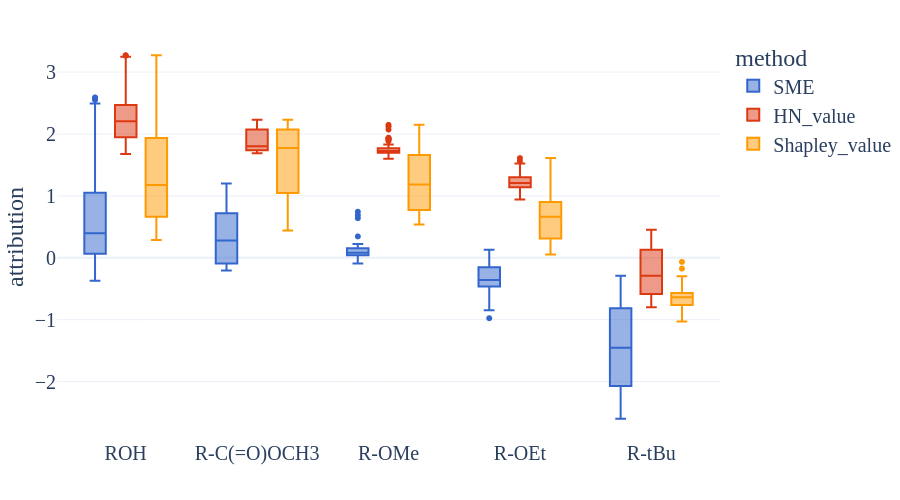
\includegraphics[scale=0.5]{attribution_distribution_functional_groups.png}
    \caption{The Shapley value, HN value, and SME attribution distributions for selected functional groups.}
    \label{fig:attribution_distribution_fg}
\end{figure}


Shapley values have mostly a broader IQR relative to the HN values. The median 
Shapley value of alcohols is lower than methyl esters, which is unexpected. 
However, SME assigns negative attributions to hydroxyl groups, which incorrectly suggests 
that hydroxyl groups can decrease the solubility of small molecules. One of those 
molecules is erythritol (\cref{fig:erythritol_explanation}), which has a predicted solubility of 0.432 log(mol/L) 
and an experimental solubility of 0.700 log(mol/L). Since the absolute prediction 
error is within acceptable limits, it would be possible that the model achieved 
this in a chemically incorrect way (i.e. clever Hans effect\cite{lapuschkin2019unmasking}). The clever Hans 
effect is supported by the wrong Shapley value explanation as it gives the 
apolar carbon chain a higher attribution than the hydroxyl groups. However, 
the explanation of the HN values is chemically correct, which makes it difficult 
to judge whether there is a clever Hans effect. 

Furthermore, the absolute prediction 
error for only five of the sixteen molecules with a negative SME attribution for 
hydroxyl groups is greater than the experimental error. However, those five molecules 
have a chemically consistent explanation from Shapley and HN values. The fact that only 
five of the wrong SME explanations are indeed wrongly predicted and the other attribution 
are in agreement with chemical theory tends to show that SME does not provide the correct 
model explanation. To obtain better understanding of the agreement/disagreement between 
attribution methods and the relation with absolute prediction error, a ranked based analysis is performed. 


\begin{figure}[h]
    \centering
    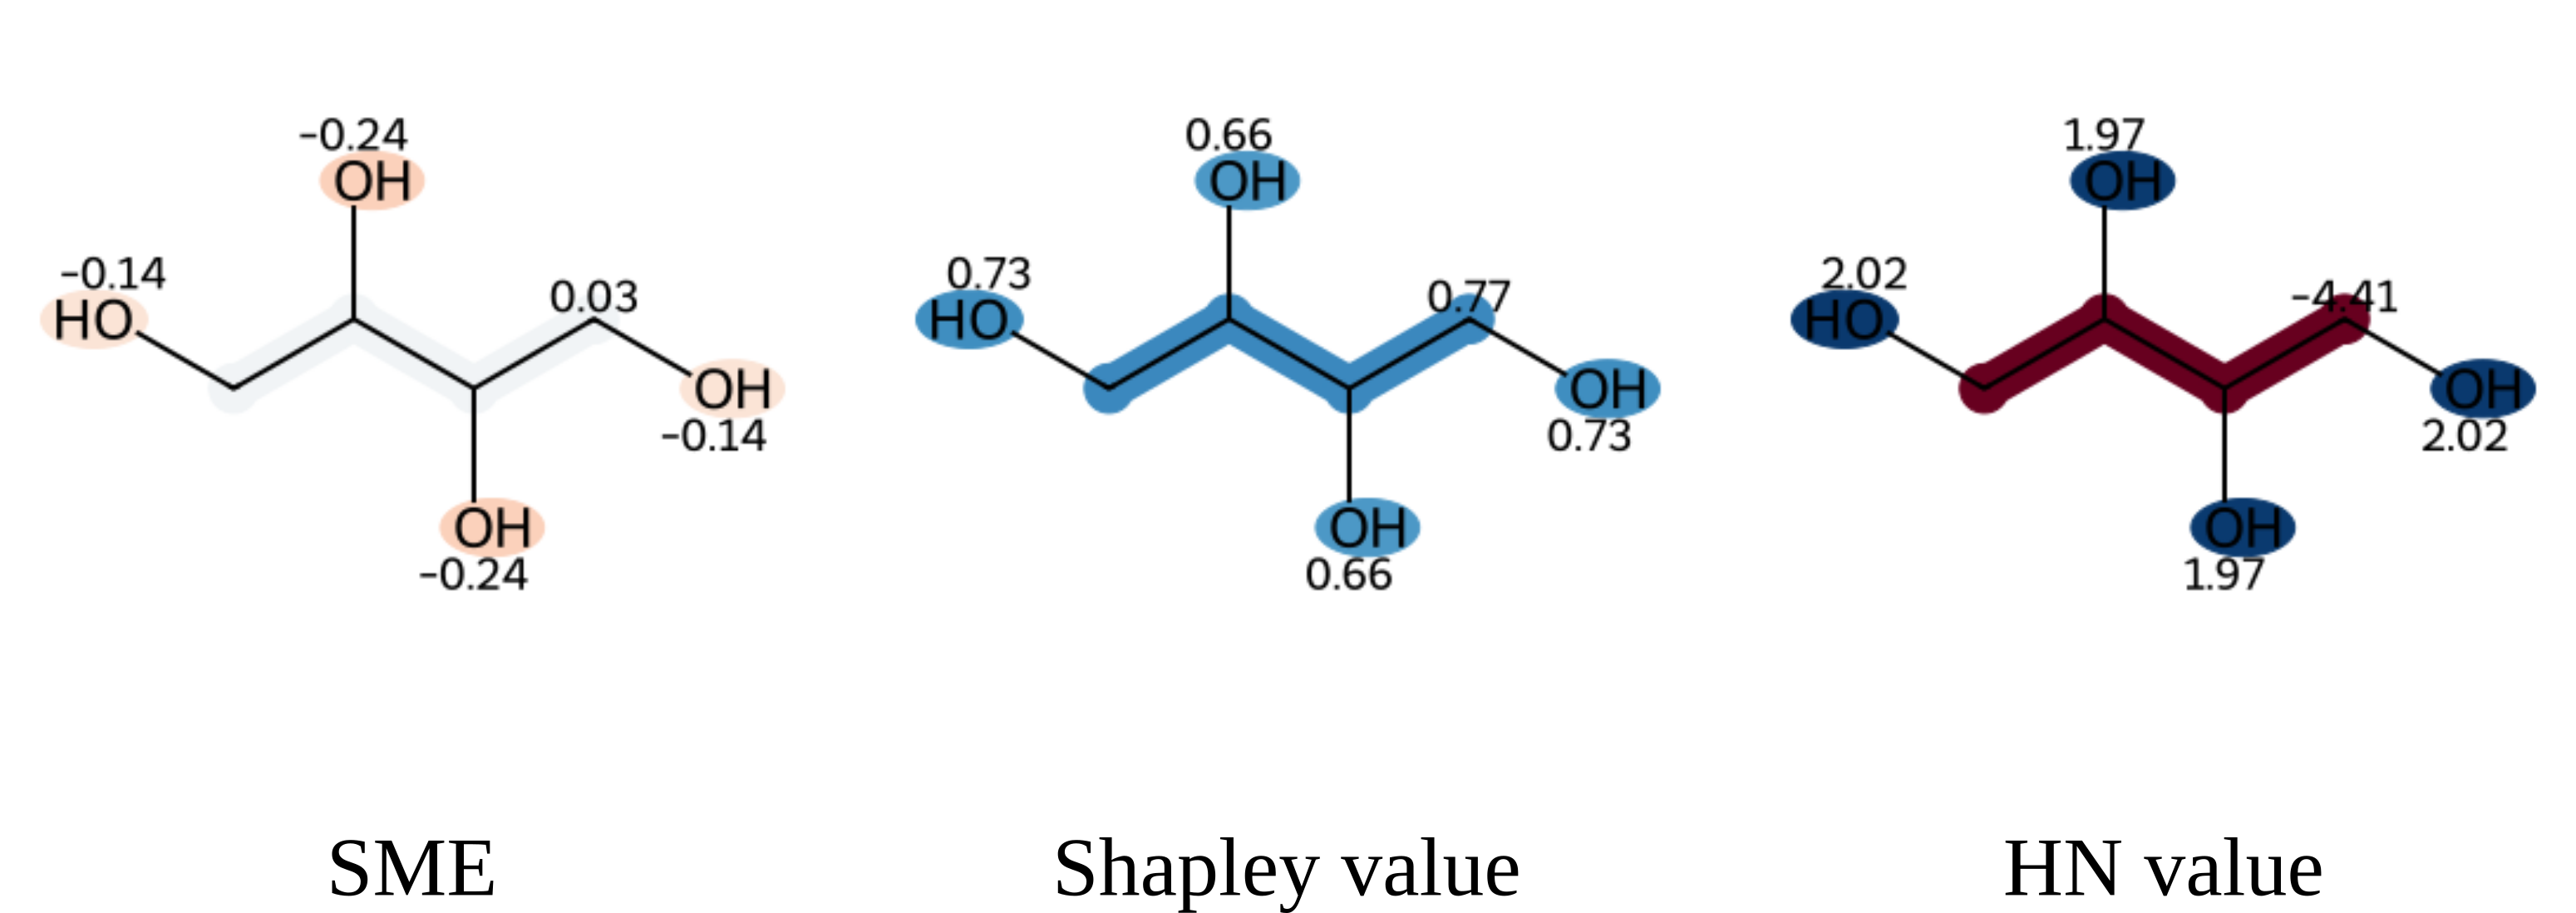
\includegraphics[scale=0.85]{erythritol_explanations.png}
    \caption{Explanations of erythritol: SME is wrong due to the negative attributions on the hydroxyl groups, 
    Shapley values are wrong since hydroxyl groups have a lower attribution than the carbon chain, HN values provide 
    a chemically correct explanation. Predicted solubility is 0.432 log(mol/L) and the experimental water solubility is 
    0.700 log(mol/L).}
    \label{fig:erythritol_explanation}
\end{figure}


\section{The absolute prediction error is not associated with the Spearman rank correlation between different attribution methods}


% To get more insight into how much the different attribution method agree/disagree 
% with each other and wheter disagreement can be explained by the absolute prediction 
% error, a ranked based approach is used. All substructures are ranked from low attributions 
% (i.e. most hydrophobic) towards high attributions (i.e. most hydrophylic). Subsequently,
% the Pearson correlation is computed between the ranks of two attribution methods. 


\begin{figure}[h]
    \centering
    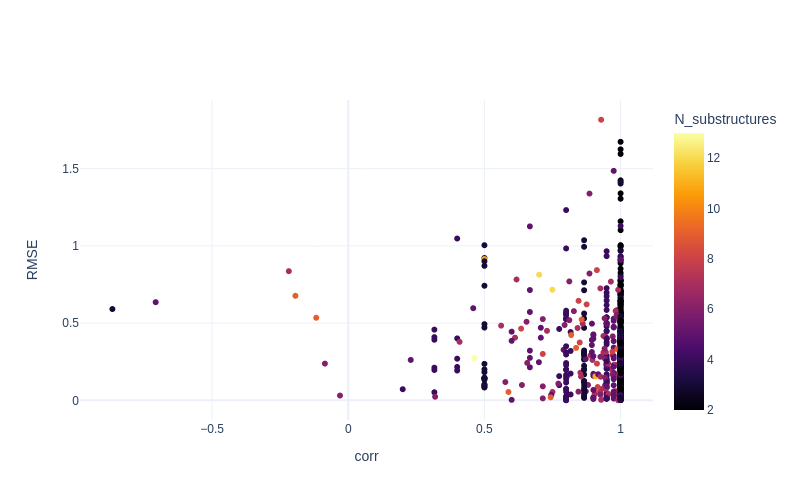
\includegraphics[scale=0.35]{../data/images/esol_rank_vs_AE_SME_Shapley_combined.png}
    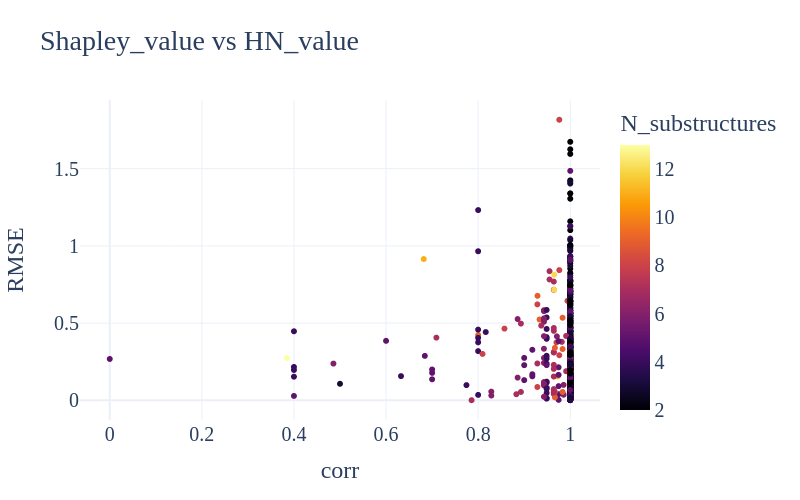
\includegraphics[scale=0.35]{../data/images/esol_rank_vs_AE_Shapley_HN_combined.png}
    \caption{Absolute error of model prediction in function of Spearman rank correlation between 
        attributions from SME and Shapley (top) and between Shapley and HN (bottom) using the full 
        data set containing 1110 molecules.
    }
\end{figure}


\section{Relative evaluation of attribution methods using chemically intuitively ranked substructures shows no statistical
significant difference between the attribution methods}

\begin{figure}[h]
    \centering
    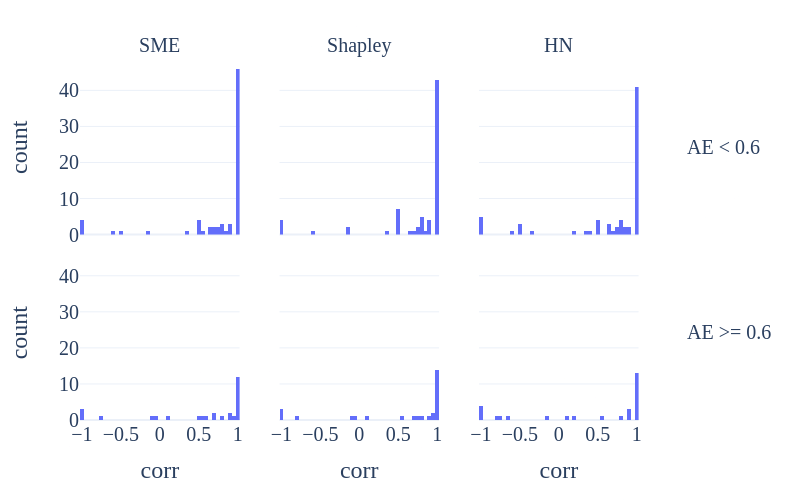
\includegraphics[scale=0.5]{spearman_rank_correlation_manual_vs_attribution.png}
    \caption{Distribution of Spearman rank correlation between an attribution method 
        and a manual ranking of substructures using chemical reasoning. The difference 
        between the two absolute error groups is mainly the intensity of high 
        correlation values.
    }
    \label{fig:spearman_corr_manual}
\end{figure}


\section{All attribution methods are equally faithful to the ML model}

\begin{figure}[h]
    \centering
    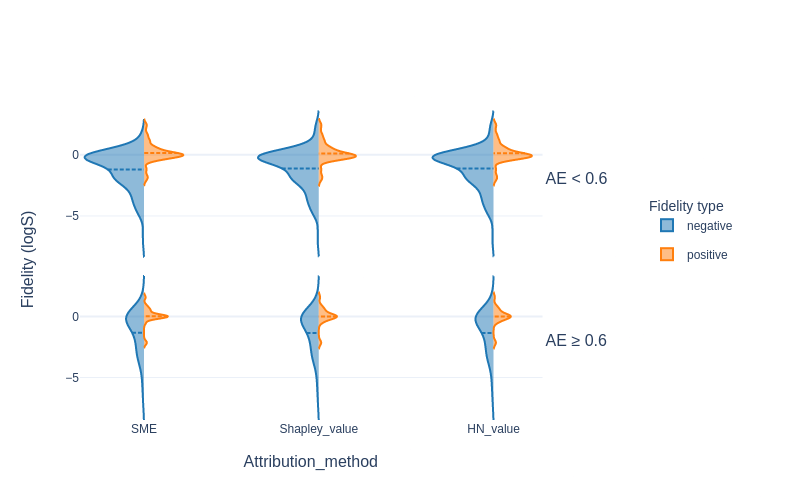
\includegraphics[scale=0.5]{fidelity.png}
    \caption{Distribution of fidelity obtained by removing the most positive 
        attribution (right side) or the most negative attribution (left side).
    }
    \label{fig:fidelity}
\end{figure}


\begin{figure}[h]
    \centering
    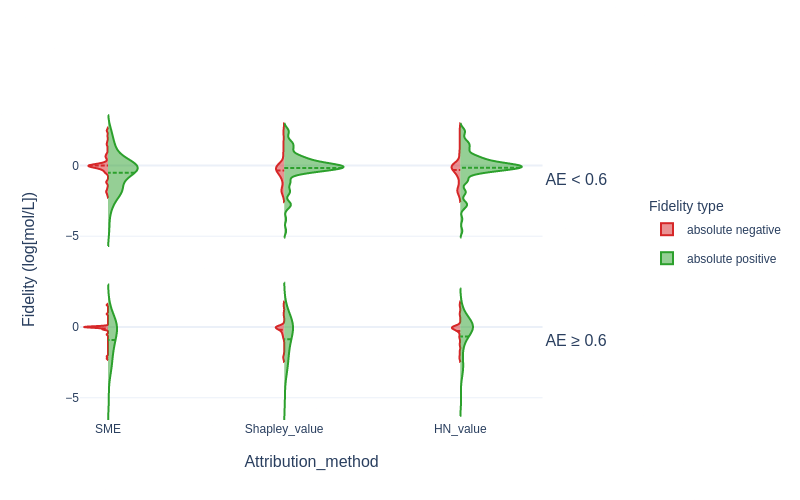
\includegraphics[scale=0.5]{absolute_fidelity.png}
    \caption{Distribution of fidelity obtained by removing the most positive 
        attribution in absolute values (right side) or the most negative 
        attribution in absolute values (left side).
    }
    \label{fig:fidelity}
\end{figure}
